\begin{figure}[H]
\centering
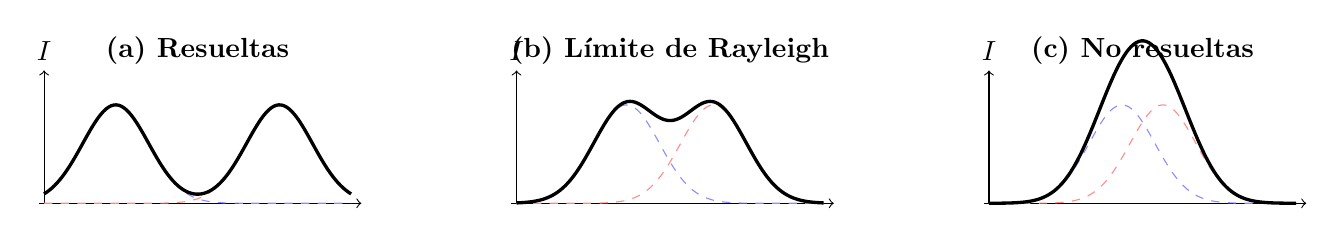
\begin{tikzpicture}[x=0.65cm,y=1.25cm]
  \foreach \shift/\sep/\titulo in {0/3.2/{(a) Resueltas},6.0/1.7/{(b) Límite de Rayleigh},12.0/0.8/{(c) No resueltas}}{
    \begin{scope}[xshift=\shift cm]
      \draw[->] (-3.1,0) -- (3.2,0);
      \draw[->] (-3,0) -- (-3,1.35) node[above] {$I$};
      \draw[blue!45,dashed,domain=-3:3,samples=100,smooth]
        plot (\x,{exp(-1.2*(\x+\sep/2)^2)});
      \draw[red!45,dashed,domain=-3:3,samples=100,smooth]
        plot (\x,{exp(-1.2*(\x-\sep/2)^2)});
      \draw[black,very thick,domain=-3:3,samples=120,smooth]
        plot (\x,{exp(-1.2*(\x+\sep/2)^2)+exp(-1.2*(\x-\sep/2)^2)});
      \node[font=\bfseries] at (0,1.55) {\titulo};
    \end{scope}
  }
\end{tikzpicture}
\caption{Perfiles de intensidad para dos fuentes: resueltas, en el límite de Rayleigh y no resueltas.}
\end{figure}